\section{Motivating Example}
\label{sec:background}

% 我们首先基于例子和模型中算子的性能评测数据的说明本工作的设计目标。
% 接下来，我们讨论挑战。
% 最后，我们介绍 \mysys 的核心设计动机。


% 重新总结 \section{Motivating  Example} 这一节：

% 1. 首先给出一个subsection，综合阐述基于跨DL系统软件栈的常量传播。首先是一个subsubsection，介绍对 DL 系统全栈的常量值传递过程。利用我给出的第一个图，首先展示 DL system 调用算子过程中的常量值传播的流程，揭示出当模型架构确定时，核函数通常有参数是运行时的不变量，例如图中的stages参数。然后再用一个subsubsection，展示算子库中现在的瓶颈和常量传播的优化机会。图2分别给出了我们统计的CANN这种generic（非特化）的算子库在推理LLM时的主要算子的评测数据，在控制流处理和标量计算方面存在一定的性能瓶颈。图3给出了我们统计的主要算子核函数参数中变量和常量的数目，反映出大部分核函数参数是运行时的不变量，揭示了：只特化这些运行时不变量的参数就有机会缓解图2展示的性能问题，同时可以保证正确性。核心关键是推导出哪些参数是运行时不变量，以及对应的值。

% 2. 接下来，再给出下一个subsection，揭示为什么需要一个新的常量信息传播框架，而不能参考现有的算子特化方法？第一个subsubsection，简单介绍一下 AI 加速器的区别，简单比较 GPU 和 Ascend 架构的差异。基于图4说明在Ascend这种可编程部件很多的硬件架构上，每层计算和访存部件都需要一些调度参数来控制运行时的流水并行。例如flash attention，每种类型的子任务（图4中的方框）都需要被指定调度参数，导致核函数的参数数目很多。参考图3。在这种背景下，现有的调用算子的方法，基于Triton/TVM 这类 AI Compiler 的方法需要基于 High-level IR 描述计算，能力依然受限，不能完全取代手写算子库，且需要运行时生成特化算子，引入额外编译开销。基于手工特化的算子库，需要在开发阶段手动枚举模板实例，此时由于模型架构、目标硬件不确定，需要为各种可能的模型、不同硬件配置提前枚举各种可能的实例。这导致严重的代码膨胀。 尤其对于 Ascend 的参数数目多的算子，手动预先枚举实例是几乎无法做到的。

% 3. 接下来，再有一个subsection，介绍Challenges，主要是两点：Propagating constant informations through Python/C++ Bindings 和 Sanity Checks leading to Early Return Paths。

% 4. 最后的一个 subsection，介绍 Design Insights of \mysys。

\begin{figure}[htbp]
    \centering
    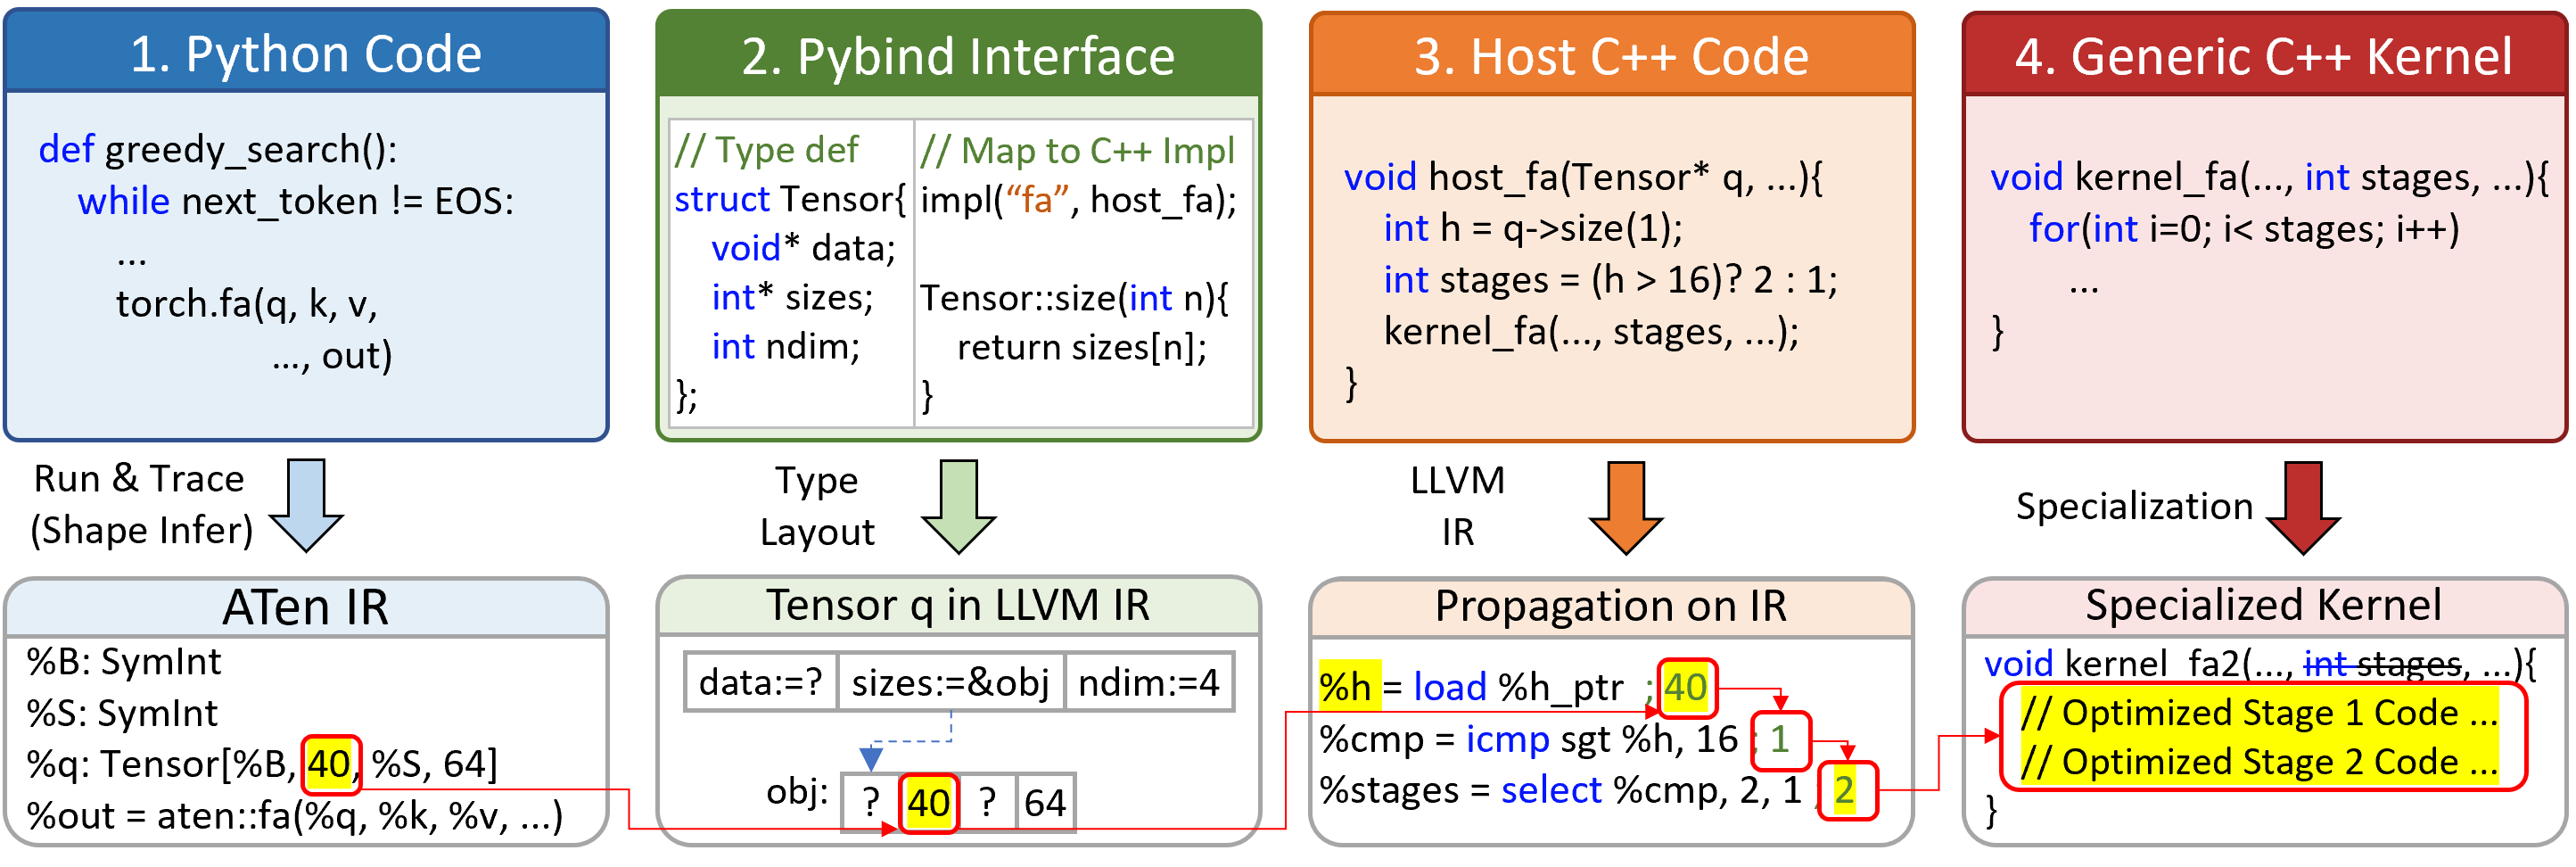
\includegraphics[width=\linewidth]{figures/motivation/motivating-example.png}
    \caption{A simplified example of a real-world DL model illustrating value flows across Python and C++ languages, and the final constants can be used to specialize kernel function, i.e. \texttt{kernel\_fa}.}
    \label{fig:motivating-example}
\end{figure}

\subsection{Ascend Architecture}

The Ascend~\cite{liao2019davinci} processor is a representative SIMD-based deep learning accelerator that adopts a decoupled architecture to separate control from computation. 
Ascend comprises three primary programmable components organized in a hierarchical manner:

\begin{itemize}
    \item \textbf{Scalar unit:} Situated at the top of the control hierarchy, it serves as the central processing unit responsible for flow control, address calculation, and instruction dispatch to other units.
    \item \textbf{Vector Unit:} A SIMD execution unit designed for element-wise operations and vector reductions.
    \item \textbf{Cube Unit:} A specialized matrix multiplication accumulation (MMA) unit designed to accelerate high-density GEMM operations.
\end{itemize}

Complementing these compute units is a sophisticated software-managed memory hierarchy. 
It includes high-speed on-chip buffers: the \textit{Unified Buffer (UB)} serving the Vector/Scalar units, and \textit{L0 Buffers} dedicated to the Cube unit. 
These are backed by large-capacity \textit{Global Memory (GM)} and L2 cache. 
A critical feature of this architecture is that data movement between these levels and layout transformations (e.g., linear \textit{ND} to fractal \textit{NZ}) must be explicitly managed by kernel instructions.

High-performance operators like \textbf{Flash Attention}~\cite{dao2024flashattention2} exemplify the scheduling complexity on this architecture. 
As shown in the green box of \autoref{fig:fa_on_ascend}, the execution follows a \textit{Tiled Loop} pipeline that interleaves heterogeneous computation. 
Matrix multiplications are performed by Cube units (e.g., $Q \times K^T$), while intermediate results are transferred to Vector units for vectorized operations (e.g., Softmax). 
This process necessitates frequent, synchronized data transfers between the GM, UB, and L0 buffers.

To orchestrate this complex pipeline, the kernel must manage a vast set of \textit{schedule parameters} (e.g., tiling sizes, memory offsets, and stride information) for every specific data movement and computation step.
Since input shapes vary at runtime, these parameters cannot be totally fixed at compile time. 
They must be passed as dynamic arguments (bottom-left of \autoref{fig:fa_on_ascend}).
Crucially, as depicted by the red dashed lines in \autoref{fig:fa_on_ascend}, the Scalar unit acts as the micro-manager of this loop. 
In each iteration, it must calculate precise memory addresses based on these parameters and dispatch control signals to trigger data movement (e.g., $Q_{GM} \to Q_{tile}$) and computation (e.g., MatMul).
Consequently, for operators with small tile sizes or complex implementations, the Scalar unit may become overloaded by these dense index calculations and dispatching tasks. 
This overload may prevent it from issuing instructions fast enough to keep the massive Cube and Vector units busy, leading to pipeline stalls and suboptimal hardware utilization.

\begin{figure}[htbp]
  \centering
  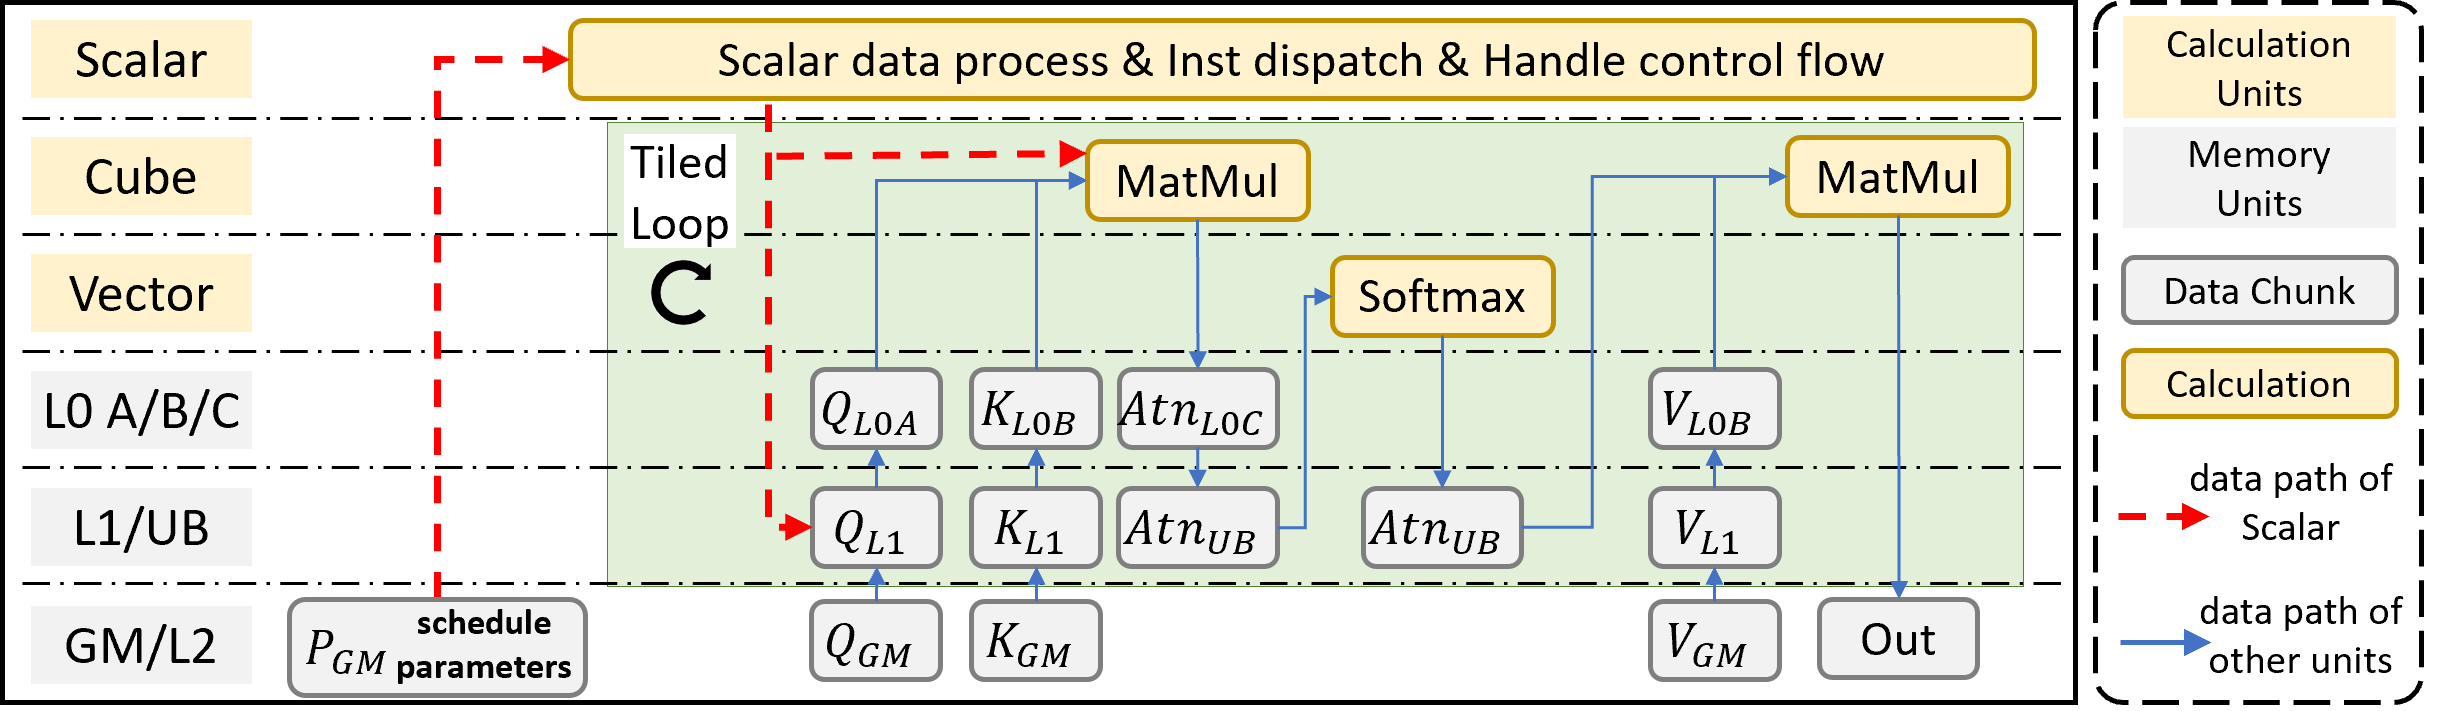
\includegraphics[width=0.8\textwidth]{figures/motivation/ascend-data-path.png}
  \caption{Execution flow of Flash Attention on the Ascend architecture. The \textbf{Scalar unit} acts as the central scheduler. It continuously calculates indices and dispatches instructions (red dashed lines) to coordinate the \textbf{Tiled Loop} of data movement (blue solid lines) and computation based on runtime parameters. The heavy scalar workload may lead to the scalar bottleneck.}
  \Description{}
  \label{fig:fa_on_ascend}
\end{figure}

\subsection{Kernel Specialization based on Template Kernels}

Modern AI compiler frameworks, such as TVM~\cite{chen2018tvm}, Triton~\cite{tillet2019triton}, BladeDISC~\cite{zheng2023bladedisc}, XLA~\cite{tensorflow2021xla} and Inductor~\cite{ansel2024dynamo}, extensively utilize template-based mechanisms or parameterized code generation to achieve kernel specialization. 
In these systems, high-performance kernels are structured as generic templates, with performance-critical arguments, such as tiling sizes and other control-flow-dependent arguments, defined as compile-time tunable parameters.
To generate executable binaries, these systems typically adopt one of two compilation paradigms:

\textbf{JIT specialization.} 
JIT-based frameworks (e.g., Triton, TVM) perform kernel specialization at runtime. 
During execution, they employ strategies like \textit{autotuning}~\cite{chen2018autotvm,zheng2020ansor} to determine the optimal tunable parameters for the current input shape, and then trigger the compiler backend to generate a specialized kernel (as shown in \kw{jit\_add} in \autoref{lst:compare_aot_jit}).
While this approach ensures specialization on demand, it introduces severe runtime compilation overhead.

\textbf{AoT specialization.}
Alternatively, compilers can specialize kernels ahead of time, e.g., FlashInfer's AOT mode~\cite{ye2025flashinfer}, generating specialized kernels before execution.
However, since the specific static information (e.g., hidden sizes, maximum context length) of the target model is often unknown or variable at library build time, these compilers must employ an exhaustive enumeration strategy.
They generate kernels for a wide range of possible template parameter combinations (e.g., enumerating all common tile sizes) to cover potential runtime scenarios (as shown in \kw{aot\_add}).
This leads to significant binary bloat, as the vast majority of these pre-generated specialized kernels are never invoked by the specific model at runtime, resulting in substantial storage and memory waste.

\begin{figure}[htbp]
\begin{minipage}{0.51\textwidth}
\begin{lstlisting}[basicstyle=\ttfamily\footnotesize, captionpos=b, frame=single]
template <int T>
void kernel(float* A, float* B, float* C, int s);

// JIT: Generate and compile code at runtime
status jit_add(Tensor& A, ...) {
  // Runtime Profiling
  int best_T = profile(A);
  compile_and_run(kernel, best_T, A, ...);
}
\end{lstlisting}
\end{minipage}
\hfill
\begin{minipage}{0.45\textwidth}
\begin{lstlisting}[firstnumber=10, basicstyle=\ttfamily\footnotesize, captionpos=b, frame=single]
// AoT: Enumeration
status aot_add(Tensor& A, ...) {
  int t = 0; tiling(A.size(0), t);
  switch (t) {
    case 16: kernel<16>(...); break;
    case 32: kernel<32>(...); break;
    case 64: kernel<64>(...); break;
    // ... dozens of cases ...
}}
\end{lstlisting}
\end{minipage}
\caption{Comparison of AoT and JIT specialization mechanisms.}
\label{lst:compare_aot_jit}
\end{figure}

\subsection{Static Analysis for Constant Propagation}

Constant propagation is a compiler optimization that identifies values known at compile-time and maps variables with runtime valuess. 
Two standard techniques are widely used:

\begin{itemize}
    \item \textbf{Data Flow Analysis(DFA):} DFA~\cite{wegman1991sccp,callahan1986icp,Sui2016SVFInterproceduralStatic} propagates information through the Control Flow Graph (CFG) using lattice~\cite{Kildall1973lattice} (e.g., \textit{Top}, \textit{Constant}, \textit{Bottom}) or value range~\cite{patterson1995valuerange}. 
    It iteratively updates the variable states until a fixed point is reached.
    Existing standard DFA-based methods are efficient but typically \textit{path-insensitive}, meaning they merge information across branches, which may lead to precision loss (i.e., values degrading to \textit{Bottom}) when control flow merges.
    
    \item \textbf{Symbolic Execution(SE):} SE~\cite{Cadar2008KLEEUnassistedAutomatic,Yao2024FalconFusedApproach} explores program paths individually, maintaining execution states as symbolic constraints. 
    It is \textit{path-sensitive} and highly precise, as it can distinguish values across different execution paths. 
    However, it faces the path explosion problem, making it computationally expensive for large or complex programs.
\end{itemize}

These techniques form the foundation of modern compiler optimization but are traditionally designed for single-language analysis contexts (e.g., pure C++).